\documentclass[11pt]{article}
\usepackage[a4paper,top=2cm,bottom=3cm,left=1.5cm,right=1.5cm]{geometry}
\usepackage{titling}
\usepackage{amsmath}
\usepackage{amssymb}
\usepackage{amsthm}
\usepackage{tikz}
\usepackage{thmtools}
\usepackage[shortlabels]{enumitem}
\usepackage{abstract}
\usepackage{hyperref}

\title{Special Topics on Graph Algorithms}
\date{Spring 2021}

% bold math
\makeatletter
\g@addto@macro\bfseries{\boldmath}
\makeatother

% remove abstract title
\renewcommand{\abstractname}{}
\renewcommand{\absnamepos}{empty}

% style of links
\hypersetup{colorlinks,linkcolor=black}

% set theorem style
\declaretheoremstyle[
  spaceabove=6pt, spacebelow=6pt,
  headfont=\normalfont\bfseries,
  notefont=\normalfont\bfseries,
  bodyfont=\normalfont\upshape,
  postheadspace=0.5em
]{custom}

% set qed symbol
\renewcommand{\qedsymbol}{$\blacksquare$}

% types of theorems
\declaretheorem[style=custom,parent=section]{definition}
\declaretheorem[style=custom,sibling=definition]{example}
\declaretheorem[style=custom,sibling=definition]{theorem}
\declaretheorem[style=custom,sibling=definition]{fact}
\declaretheorem[style=custom,sibling=definition]{algorithm}

% use bold fonts to emphasize
\DeclareTextFontCommand{\emph}{\bfseries}

\newcommand{\NN}{\mathbb{N}}
\newcommand{\ZZ}{\mathbb{Z}}
\newcommand{\QQ}{\mathbb{Q}}
\newcommand{\RR}{\mathbb{R}}

\begin{document}

% title
\begin{center}
  \LARGE \bfseries \thetitle, \thedate
\end{center}

\begin{abstract}
  This note is taken for the course "Special Topics on Graph Algorithms", which is instructed by Kun-Mao Chao in Spring 2021.
\end{abstract}

\tableofcontents

\section{February 23, 2021}
\subsection{Course Introduction}
This course will mostly focus on tree-related problems with their applications.
\begin{itemize}
  \item Scoring: Midterm exams ($35\%+35\%$), oral representation ($20\%$), and class participation ($10\%$).
  \item Textbook: \textsl{Spanning Trees and Optimization Problems}, by Bang Ye Wu and Kun-Mao Chao (2004).
\end{itemize}

\subsection{Number of Spanning Trees of $K_n$}
A \emph{spanning tree} of a graph $G$ is a subgraph of $G$ that is a tree which contains all vertices of $G$.
Let $K_n$ denote the complete graph on the $n$ vertices $\{1, 2, \dots, n\}$.

\begin{example}
  The number of spanning trees of $K_4$ is $16$.
  \begin{figure}[h]
    \centering
    \begin{minipage}{0.17\textwidth}
      \begin{tikzpicture}[every node/.style={fill,circle,minimum size=4pt,inner sep=0}]
        \node[label={[shift={(0.15,0.05)},font=\scriptsize]1}] (1) at (0,0) {};
        \node[label={[shift={(0,0.1)},font=\scriptsize]2}] (2) at (0,1.15) {};
        \node[label={[shift={(-0.25,-0.4)},font=\scriptsize]3}] (3) at (-1,-0.58) {};
        \node[label={[shift={(0.25,-0.4)},font=\scriptsize]4}] (4) at (1,-0.58) {};
        \draw (1) -- (2) (1) -- (3) (1) -- (4);
      \end{tikzpicture}
    \end{minipage}
    \begin{minipage}{0.17\textwidth}
      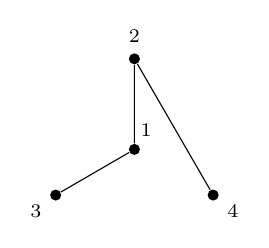
\begin{tikzpicture}[every node/.style={fill,circle,minimum size=4pt,inner sep=0}]
        \node[label={[shift={(0.15,0.05)},font=\scriptsize]1}] (1) at (0,0) {};
        \node[label={[shift={(0,0.1)},font=\scriptsize]2}] (2) at (0,1.15) {};
        \node[label={[shift={(-0.25,-0.4)},font=\scriptsize]3}] (3) at (-1,-0.58) {};
        \node[label={[shift={(0.25,-0.4)},font=\scriptsize]4}] (4) at (1,-0.58) {};
        \draw (1) -- (2) (1) -- (3) (2) -- (4);
      \end{tikzpicture}
    \end{minipage}
    \begin{minipage}{0.17\textwidth}
      \begin{tikzpicture}[every node/.style={fill,circle,minimum size=4pt,inner sep=0}]
        \node[label={[shift={(0.15,0.05)},font=\scriptsize]1}] (1) at (0,0) {};
        \node[label={[shift={(0,0.1)},font=\scriptsize]2}] (2) at (0,1.15) {};
        \node[label={[shift={(-0.25,-0.4)},font=\scriptsize]3}] (3) at (-1,-0.58) {};
        \node[label={[shift={(0.25,-0.4)},font=\scriptsize]4}] (4) at (1,-0.58) {};
        \draw (1) -- (2) (1) -- (3) (3) -- (4);
      \end{tikzpicture}
    \end{minipage}
    \begin{minipage}{0.17\textwidth}
      \begin{tikzpicture}[every node/.style={fill,circle,minimum size=4pt,inner sep=0}]
        \node[label={[shift={(0.15,0.05)},font=\scriptsize]1}] (1) at (0,0) {};
        \node[label={[shift={(0,0.1)},font=\scriptsize]2}] (2) at (0,1.15) {};
        \node[label={[shift={(-0.25,-0.4)},font=\scriptsize]3}] (3) at (-1,-0.58) {};
        \node[label={[shift={(0.25,-0.4)},font=\scriptsize]4}] (4) at (1,-0.58) {};
        \draw (1) -- (2) (1) -- (4) (3) -- (4);
      \end{tikzpicture}
    \end{minipage}
    \\
    \begin{minipage}{0.17\textwidth}
      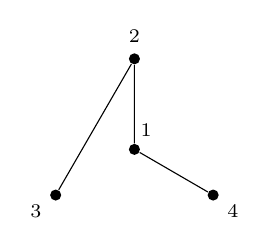
\begin{tikzpicture}[every node/.style={fill,circle,minimum size=4pt,inner sep=0}]
        \node[label={[shift={(0.15,0.05)},font=\scriptsize]1}] (1) at (0,0) {};
        \node[label={[shift={(0,0.1)},font=\scriptsize]2}] (2) at (0,1.15) {};
        \node[label={[shift={(-0.25,-0.4)},font=\scriptsize]3}] (3) at (-1,-0.58) {};
        \node[label={[shift={(0.25,-0.4)},font=\scriptsize]4}] (4) at (1,-0.58) {};
        \draw (1) -- (2) (1) -- (4) (2) -- (3);
      \end{tikzpicture}
    \end{minipage}
    \begin{minipage}{0.17\textwidth}
      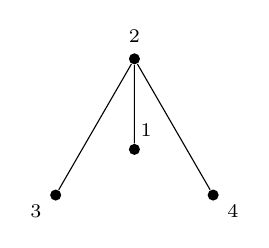
\begin{tikzpicture}[every node/.style={fill,circle,minimum size=4pt,inner sep=0}]
        \node[label={[shift={(0.15,0.05)},font=\scriptsize]1}] (1) at (0,0) {};
        \node[label={[shift={(0,0.1)},font=\scriptsize]2}] (2) at (0,1.15) {};
        \node[label={[shift={(-0.25,-0.4)},font=\scriptsize]3}] (3) at (-1,-0.58) {};
        \node[label={[shift={(0.25,-0.4)},font=\scriptsize]4}] (4) at (1,-0.58) {};
        \draw (1) -- (2) (2) -- (3) (2) -- (4);
      \end{tikzpicture}
    \end{minipage}
    \begin{minipage}{0.17\textwidth}
      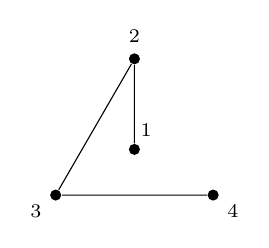
\begin{tikzpicture}[every node/.style={fill,circle,minimum size=4pt,inner sep=0}]
        \node[label={[shift={(0.15,0.05)},font=\scriptsize]1}] (1) at (0,0) {};
        \node[label={[shift={(0,0.1)},font=\scriptsize]2}] (2) at (0,1.15) {};
        \node[label={[shift={(-0.25,-0.4)},font=\scriptsize]3}] (3) at (-1,-0.58) {};
        \node[label={[shift={(0.25,-0.4)},font=\scriptsize]4}] (4) at (1,-0.58) {};
        \draw (1) -- (2) (2) -- (3) (3) -- (4);
      \end{tikzpicture}
    \end{minipage}
    \begin{minipage}{0.17\textwidth}
      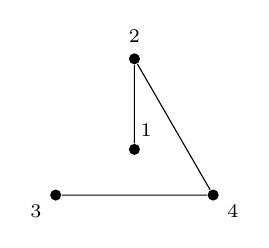
\begin{tikzpicture}[every node/.style={fill,circle,minimum size=4pt,inner sep=0}]
        \node[label={[shift={(0.15,0.05)},font=\scriptsize]1}] (1) at (0,0) {};
        \node[label={[shift={(0,0.1)},font=\scriptsize]2}] (2) at (0,1.15) {};
        \node[label={[shift={(-0.25,-0.4)},font=\scriptsize]3}] (3) at (-1,-0.58) {};
        \node[label={[shift={(0.25,-0.4)},font=\scriptsize]4}] (4) at (1,-0.58) {};
        \draw (1) -- (2) (2) -- (4) (3) -- (4);
      \end{tikzpicture}
    \end{minipage}
    \\
    \begin{minipage}{0.17\textwidth}
      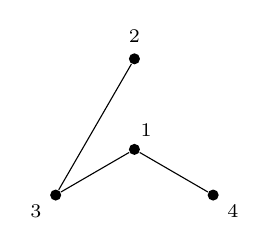
\begin{tikzpicture}[every node/.style={fill,circle,minimum size=4pt,inner sep=0}]
        \node[label={[shift={(0.15,0.05)},font=\scriptsize]1}] (1) at (0,0) {};
        \node[label={[shift={(0,0.1)},font=\scriptsize]2}] (2) at (0,1.15) {};
        \node[label={[shift={(-0.25,-0.4)},font=\scriptsize]3}] (3) at (-1,-0.58) {};
        \node[label={[shift={(0.25,-0.4)},font=\scriptsize]4}] (4) at (1,-0.58) {};
        \draw (1) -- (3) (1) -- (4) (2) -- (3);
      \end{tikzpicture}
    \end{minipage}
    \begin{minipage}{0.17\textwidth}
      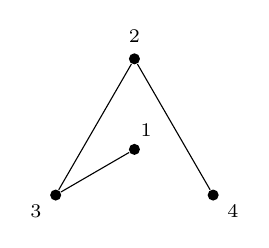
\begin{tikzpicture}[every node/.style={fill,circle,minimum size=4pt,inner sep=0}]
        \node[label={[shift={(0.15,0.05)},font=\scriptsize]1}] (1) at (0,0) {};
        \node[label={[shift={(0,0.1)},font=\scriptsize]2}] (2) at (0,1.15) {};
        \node[label={[shift={(-0.25,-0.4)},font=\scriptsize]3}] (3) at (-1,-0.58) {};
        \node[label={[shift={(0.25,-0.4)},font=\scriptsize]4}] (4) at (1,-0.58) {};
        \draw (1) -- (3) (2) -- (3) (2) -- (4);
      \end{tikzpicture}
    \end{minipage}
    \begin{minipage}{0.17\textwidth}
      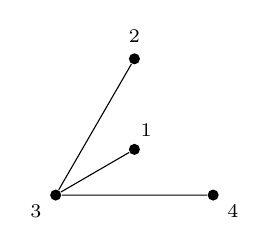
\begin{tikzpicture}[every node/.style={fill,circle,minimum size=4pt,inner sep=0}]
        \node[label={[shift={(0.15,0.05)},font=\scriptsize]1}] (1) at (0,0) {};
        \node[label={[shift={(0,0.1)},font=\scriptsize]2}] (2) at (0,1.15) {};
        \node[label={[shift={(-0.25,-0.4)},font=\scriptsize]3}] (3) at (-1,-0.58) {};
        \node[label={[shift={(0.25,-0.4)},font=\scriptsize]4}] (4) at (1,-0.58) {};
        \draw (1) -- (3) (2) -- (3) (3) -- (4);
      \end{tikzpicture}
    \end{minipage}
    \begin{minipage}{0.17\textwidth}
      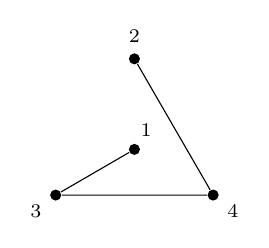
\begin{tikzpicture}[every node/.style={fill,circle,minimum size=4pt,inner sep=0}]
        \node[label={[shift={(0.15,0.05)},font=\scriptsize]1}] (1) at (0,0) {};
        \node[label={[shift={(0,0.1)},font=\scriptsize]2}] (2) at (0,1.15) {};
        \node[label={[shift={(-0.25,-0.4)},font=\scriptsize]3}] (3) at (-1,-0.58) {};
        \node[label={[shift={(0.25,-0.4)},font=\scriptsize]4}] (4) at (1,-0.58) {};
        \draw (1) -- (3) (2) -- (4) (3) -- (4);
      \end{tikzpicture}
    \end{minipage}
    \\
    \begin{minipage}{0.17\textwidth}
      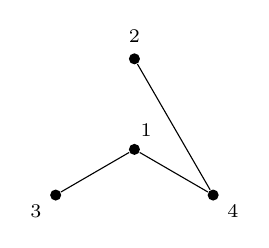
\begin{tikzpicture}[every node/.style={fill,circle,minimum size=4pt,inner sep=0}]
        \node[label={[shift={(0.15,0.05)},font=\scriptsize]1}] (1) at (0,0) {};
        \node[label={[shift={(0,0.1)},font=\scriptsize]2}] (2) at (0,1.15) {};
        \node[label={[shift={(-0.25,-0.4)},font=\scriptsize]3}] (3) at (-1,-0.58) {};
        \node[label={[shift={(0.25,-0.4)},font=\scriptsize]4}] (4) at (1,-0.58) {};
        \draw (1) -- (3) (1) -- (4) (2) -- (4);
      \end{tikzpicture}
    \end{minipage}
    \begin{minipage}{0.17\textwidth}
      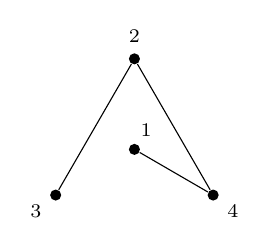
\begin{tikzpicture}[every node/.style={fill,circle,minimum size=4pt,inner sep=0}]
        \node[label={[shift={(0.15,0.05)},font=\scriptsize]1}] (1) at (0,0) {};
        \node[label={[shift={(0,0.1)},font=\scriptsize]2}] (2) at (0,1.15) {};
        \node[label={[shift={(-0.25,-0.4)},font=\scriptsize]3}] (3) at (-1,-0.58) {};
        \node[label={[shift={(0.25,-0.4)},font=\scriptsize]4}] (4) at (1,-0.58) {};
        \draw (1) -- (4) (2) -- (3) (2) -- (4);
      \end{tikzpicture}
    \end{minipage}
    \begin{minipage}{0.17\textwidth}
      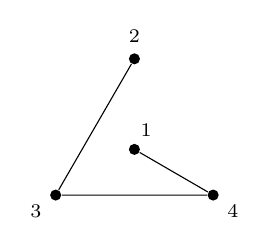
\begin{tikzpicture}[every node/.style={fill,circle,minimum size=4pt,inner sep=0}]
        \node[label={[shift={(0.15,0.05)},font=\scriptsize]1}] (1) at (0,0) {};
        \node[label={[shift={(0,0.1)},font=\scriptsize]2}] (2) at (0,1.15) {};
        \node[label={[shift={(-0.25,-0.4)},font=\scriptsize]3}] (3) at (-1,-0.58) {};
        \node[label={[shift={(0.25,-0.4)},font=\scriptsize]4}] (4) at (1,-0.58) {};
        \draw (1) -- (4) (2) -- (3) (3) -- (4);
      \end{tikzpicture}
    \end{minipage}
    \begin{minipage}{0.17\textwidth}
      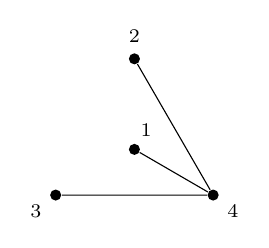
\begin{tikzpicture}[every node/.style={fill,circle,minimum size=4pt,inner sep=0}]
        \node[label={[shift={(0.15,0.05)},font=\scriptsize]1}] (1) at (0,0) {};
        \node[label={[shift={(0,0.1)},font=\scriptsize]2}] (2) at (0,1.15) {};
        \node[label={[shift={(-0.25,-0.4)},font=\scriptsize]3}] (3) at (-1,-0.58) {};
        \node[label={[shift={(0.25,-0.4)},font=\scriptsize]4}] (4) at (1,-0.58) {};
        \draw (1) -- (4) (2) -- (4) (3) -- (4);
      \end{tikzpicture}
    \end{minipage}
    \caption{All spanning trees of $K_4$.}
  \end{figure}
\end{example}

\begin{definition}
  Let $n \geq 2$.
  A \emph{Pr\"ufer sequence} is a sequence of numbers in $\{1, 2, \dots, n\}$ for some $n \geq 2$ that has length $n-2$.
\end{definition}

\begin{algorithm}[Encoding]
  Given a spanning tree $T$ of $K_n$ with $n \geq 2$, we compute the Pr\"ufer sequence $P = (p_1, p_2, \dots, p_{n-2})$ that corresponds to $T$ as follows.
  \begin{enumerate}[label=\arabic*.]
    \item For each $i \gets 1, 2, \dots, n-2$, perform the following steps.
    \begin{enumerate}[label*=\arabic*.]
      \item Let $u$ be the smallest vertex of $T$ that is a leaf, and let $v$ be the unique neighbor of $u$.
      \item Let $p_i \gets v$.
      \item Remove $u$ from $T$.
    \end{enumerate}
    \item Return $P = (p_1, p_2, \dots, p_{n-2})$.
  \end{enumerate}
\end{algorithm}

\begin{algorithm}[Decoding]
  Given a Pr\"ufer sequence $P = (p_1, p_2, \dots, p_{n-2})$, we compute the spanning tree $T$ of $K_n$ that corresponds to $P$ as follows.
  \begin{enumerate}[label=\arabic*.]
    \item Let $T$ be an empty graph on the vertices $\{1, 2, \dots, n\}$, and let $Q \gets \{1, 2, \dots, n\}$.
    \item For each $i \gets 1, 2, \dots, n-2$, perform the following steps.
    \begin{enumerate}[label*=\arabic*.]
      \item Let $u$ be the smallest vertex in $Q \setminus \{p_i, p_{i+1}, \dots, p_{n-2}\}$.
      \item Let $v \gets p_i$.
      \item Add the edge $(u, v)$ to $T$.
      \item Remove $u$ from $Q$.
    \end{enumerate}
    \item Let $u$ and $v$ be the two vertices left in $Q$.
    Add the edge $(u, v)$ to $T$.
    \item Return $T$.
  \end{enumerate}
\end{algorithm}

\begin{theorem}[Cayley's Formula]
  The number of spanning trees of $K_n$ is $n^{n-2}$.
\end{theorem}

\end{document}
